%physical principles

\section{physical principles}
\begin{figure}[H]
	\centering
	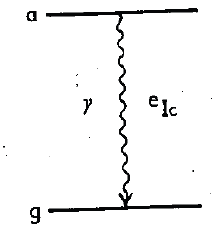
\includegraphics[height=0.18\textheight]{graphics/Emission}
	\caption[spontaneous $\gamma$ emission]{principle of spontaneous $\gamma$ emission of excited nuclei. Transitioning from an excited state ($E_a$) to the ground state ($E_g$) the nucleus emits a photon with energy $E_a-E_g=\hbar\dot \omega$ or transmits that energy directly to an electron of the atomic shell.\cite{Wegener}}
	\label{fig:principles:Emission}
\end{figure}
\subsection{Gamma Decay and and resonance Absorption}
Nuclei in excited states (energy $E_a$) can spontaneously transition into the ground (energy $E_g$) state. The energy difference $\Delta E=E_a-Eg$ is either directly gained by a shell electron (inner conversion), or carried by a emitted photon (spontaneous emission). The frequency $\omega$ of the photon is given by: 
\begin{equation}
\Delta E = h\cdot \omega
\end{equation}
where $\hbar = 6.582 119 514 \cdot 10^{-16} eVs$ is the Planck constant over $2\pi$ \cite{Codata}.
The Reverse process is also possible, namely a nucleus can transit into an excited state by absorbing a photon.

However the emission (and absorption) spectrum is not infinitely sharp, but a Lorentz distribution with natural line width $\Gamma$ (see figure \ref{fig:principles:lorentz}) \cite{Wegener}: 
\begin{equation}
I(\omega) \propto \frac{1}{(\omega-\omega_0)^2+(\Gamma /2)^2}
\label{eq:principles:Lorentz}
\end{equation}
\begin{figure}[H]
	\centering
	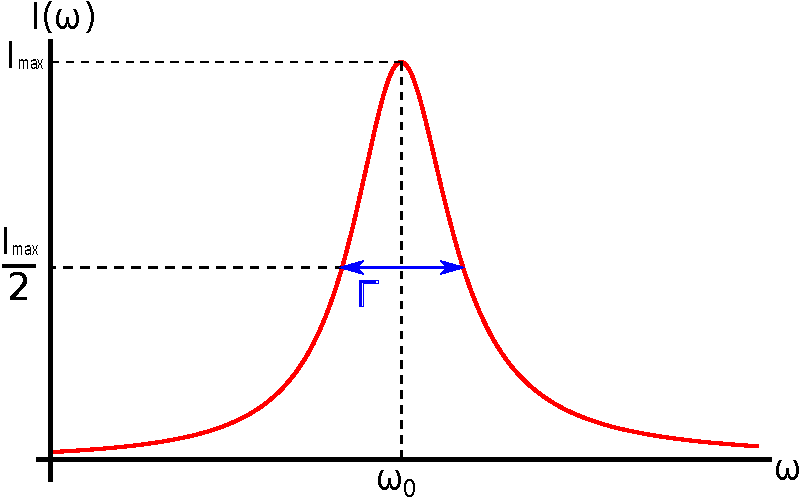
\includegraphics[height=0.25\textheight]{graphics/Lorentz.pdf}
	\caption[Lorentz distribution]{Illustration of a Lorentzian curve}
	\label{fig:principles:lorentz}
\end{figure}

 The line width is related to the mean life-time \scalebox{1.5}{$\tau$} of the excited state via Heisenberg's uncertainty relation (here energy-time uncertainty):
 
 \begin{equation}
 \hbar=\Gamma \cdot \scalebox{1.5}{$\tau$}
 \end{equation}

\subsection{Interaction of Gamma radiation with matter}
Photons interact with matter in three major ways\cite{Demtröder}:

\paragraph{Photoelectric effect} \ \\
Shell electrons of atoms absorb photons and gain its energy, leaving the potential well of the atom and exiting the shell with the energy $E_e = E_\gamma-E_B$ with $E_B$ being the binding energy of the electron.
\paragraph{Compton scattering} \ \\
Compton Scattering is the elastic scattering of photons at quasi free  electrons ($E_B << E_\gamma$) and its wavelength $\lambda=2\pi c/\omega$ shifted, depending on the scattering angle $\varphi$(see figure \ref*{eq:compton}):
\begin{equation}
\lambda_S -\lambda_0 = \frac{2 \pi \hbar}{m_e c}(1-cos(\varphi))
\label{eq:compton}
\end{equation}
\begin{figure}[h]
\centering
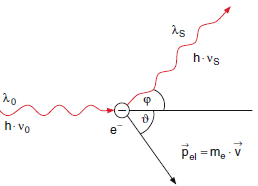
\includegraphics[width=0.5\linewidth]{graphics/Compton}
\caption{Compton effect: A photon is scattered by a (quasi) free electron changing its direction by an angle $\varphi$ }
\label{fig:principles:Compton}
\end{figure}

\subsection{Moessbauer effect}


\begin{figure}[hb]
	\centering
	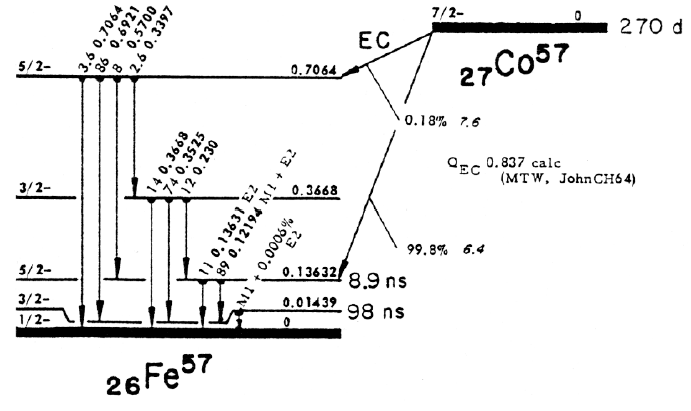
\includegraphics[width=1.0\linewidth]{graphics/Zerfallsschema}
	\caption[Co-57 decay]{decay series of Cobalt-57}
	\label{fig:principles:Zerfallsschema}
\end{figure}